\begin{frame}[fragile]{Nearest neighbor data structures for Euclidean distance}

%\begin{tikzpicture}
%\draw (-3,2) -- (9,2);
%%\draw (4,1.3) -- (8,1.3);
%\node at (0,0) {
    %\resizebox{6cm}{!}{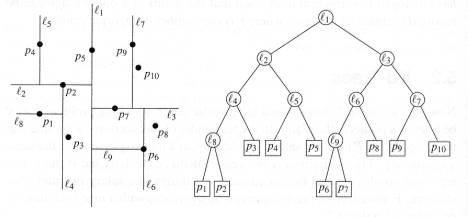
\includegraphics[width=12cm]{covertree/kdtree.jpg}}
%};
%\node at (6,1.5) { \textbf{kd-tree} };
%\node at (6,0.5) { popular in machine learning libraries };
%\node at (6,-0.5) { MLPack, scikit, R, matlab, weka };
%
%\draw (-3,-2) -- (9,-2);
%%\draw (4,-2.7) -- (8,-2.7);
%\node at (0,-4) {
    %\resizebox{6cm}{!}{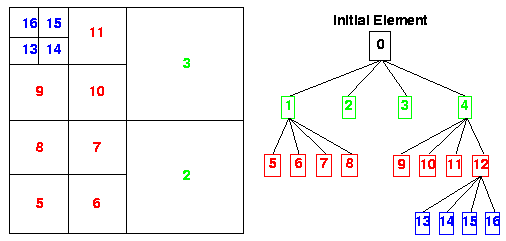
\includegraphics[width=12cm]{covertree/quadtree.png}}
%};
%\node at (6,-2.5) { \textbf{quad/oct-tree} };
%%\node at (6,-3.5) { not popular in machine learning libraries };
%\node at (6,-3.5) { mostly used in graphics };
%\node at (6,-4.5) { very bad in high dimensions };
%\draw (-3,-6) -- (9,-6);
%\end{tikzpicture}

\begin{tabular}{m{6cm}m{5.2cm}}
\hline
& \\
%\vspace{0.1in}
\resizebox{6cm}{!}{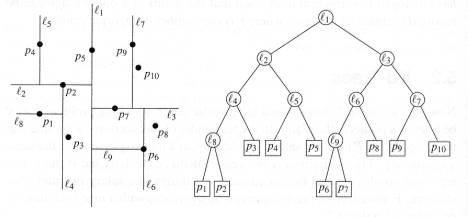
\includegraphics[width=12cm]{covertree/kdtree.jpg}} &
%\begin{tabular}{c}
%\vspace{-0.5in}
%$k$d-tree \\
%\\
%popular in machine learning: \\
%\\
%MLPack, scikit, R, matlab, weka
%\end{tabular}
%\centering
\begin{center}
\textbf{kd-tree}

popular in machine learning

MLPack, scikit, R, matlab, weka

\vspace{0.15in}
(Friedman \emph{et al.}, 1977)
\end{center}
\\
\hline
&\\
%\hline
\vspace{0.0in}
\resizebox{6cm}{!}{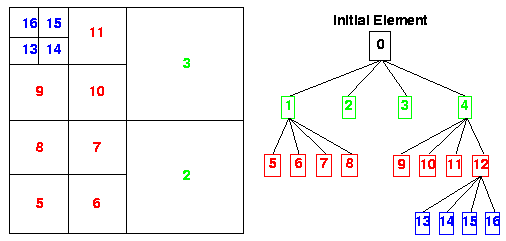
\includegraphics[width=12cm]{covertree/quadtree.png}}
\vspace{-0.12in}
&
\begin{center}
\textbf{quad/oct-tree}

not popular in machine learning
\end{center}
%\\
%\hline
%$k$d-tree & quad/oct tree\\
%popular in machine learning & \\
%(MLPack, scikit learn, R, matlab, weka, etc.)
\\
\hline
\end{tabular}

\vspace{0.1in}
{\tiny
images from: \url{http://www.cs.sandia.gov/~kddevin/LB/figs}
}

%Friedman \emph{et al.}, Transactions on Mathematical Software, 1977
%
%(2234 citations)
%
%\vspace{0.25cm}
%simple, but only works on $\mathbb{R}^n$;
%
%\vspace{0.25cm}
%
%\vspace{0.25cm}
%
% image from: http://homes.ieu.edu.tr/hakcan/projects/kdtree/files/kdtree.jpg
\end{frame}


